\subsection{Linearità di un Sistema Dinamico}%
\label{sub:Linearità di un Sistema Dinamico}
Prendiamo un sistema dinamico a tempi continui così definito:
\begin{equation}
    \frac{\text{d} \vect{x}}{\text{d} t} = F(\vect{x}, t) \qquad \vect{x}  \in \mathbb{R}^n; t \in \mathbb{R}; F: \mathbb{R}^n\times \mathbb{R} \to \mathbb{R}^n
    \label{eq:3_SD_cont}
\end{equation}
\[
    \vect{x}  = \left(x_1, x_2, \ldots, x_n\right) \qquad F = (F_1, F_2, \ldots, F_n)
.\] 
\begin{defn}[Condizione di linearità]
    \label{def:cond_lin}
    Un SD a tempi continui come quello di equazione \ref{eq:3_SD_cont} è lineare se:
    \[
	F(\vect{x}  + \vect{y}, t) = F(\vect{x}, t) + F(\vect{y}, t) \qquad \forall \vect{x}, \vect{y}  \in \mathbb{R}^n
    .\] 
\end{defn}
\noindent
Questa condizione è necessaria ma non sufficiente.
\begin{exmp}[Circuito RC]
    \marginpar{
        \captionsetup{type=figure}
        \fbox{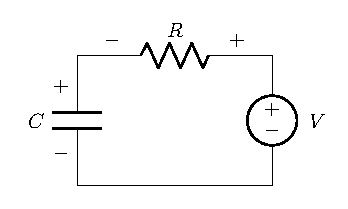
\includegraphics[width=\marginparwidth]{figures/tikz/3_rlc.pdf}}
        \caption{\scriptsize Circuito RC.}
        \label{fig:tikz-3_rlc-pdf}
    }
    Prendiamo il circuito RC come in figura \ref{fig:tikz-3_rlc-pdf}, l'equazione che regola la carica nel circuito è la seguente:
    \[
        \frac{\text{d} q}{\text{d} t} = \frac{V}{R}-\frac{q}{RC}
    .\] 
    In questo caso la variabile $x$ corrisponde con la carica.\\
    Il sistema non rispetta la condizione \ref{def:cond_lin}, infatti nello sviluppare il calcolo per due correnti, $q_1$ e $q_2$, rimane un termine $2V / R$. \\
    Nonostante questo il sistema è ancora lineare.
\end{exmp}
\noindent
\begin{exmp}[Pendolo]
    \marginpar{
        \captionsetup{type=figure}
            \incfig{1_9}
        \caption{\scriptsize }
        \label{fig:1_9}
    }
    Prendiamo il sistema del pendolo classico, le equazioni del moto della massa $m$ sono:
    \[
	\frac{\text{d} ^2\theta}{\text{d} t^2} = -\frac{g}{l}\sin\theta \implies
        \begin{cases}
	    \frac{\text{d} \theta}{\text{d} t} = y\\
	    \frac{\text{d} y}{\text{d} t} = - \frac{g}{l}\sin\theta
        \end{cases}
    .\] 
    Questo sistema è non lineare (c'è il seno).
\end{exmp}
\noindent
\begin{defn}[Criterio generale per la linearità]
    Un SD si dice lineare se la sua dipendenza dalle variabili di stato è lineare.
\end{defn}
\noindent
\section{Esistenza ed unicità della soluzione di IVP}%
\label{sub:Esistenza ed unicità della soluzione di IVP}
Dato un SD a tempo continuo ed un IVP (initial value problem) vorremmo sapere, per studiare la dinamica, se:
\begin{itemize}
    \item Il problema ha soluzione?
    \item La soluzione, se esiste, è unica?
\end{itemize}
In assenza di unicità il sistema non può essere deterministico. I sistemi dinamici che studiamo devono sempre essere deterministici.
\begin{exmp}[Due soluzioni]
    \[
        \begin{cases}
	    \frac{\text{d} x}{\text{d} t} = 3x^{2 /3} = F(x)\\
	    x(0)=x_0=0
        \end{cases}
    .\] 
    Il sistema non è lineare poiché
    \[
        \left(x+y\right)^{2 /3} \neq x^{2 /3}+y^{2 /3}
    .\] 
    Possiamo subito notare che una prima soluzione è la nulla: $x_1(t)=0$.
    Un'altra soluzione è invece $x_2(t)=t^3$, infatti sostituendo nella equazione per la derivata di $x$:
    \[
	3t^2 = 3(t^3)^{2 /3}
    .\] 
    Che è appunto verificata. \\
    Possiamo notare che $F(x)$ è continua in $x_0$, tuttavia non lo è la sua derivata rispetto a $x$: diverge a $\pm \infty$. Questo fatto è strettamente correlato alla non unicità della soluzione.
\end{exmp}
\noindent
La non unicità della soluzione non è l'unico problema nel caso di sistemi dinamici a tempo continuo, può anche accadere che la soluzione non esista per tutti i tempi $\in \mathbb{R}$.
\begin{exmp}[Soluzione con discontinuità nel tempo]
    \[
        \begin{cases}
	    \frac{\text{d} x}{\text{d} t} = x^2=F(x)\\
	    x(0)=1
        \end{cases}
    \] 
    In questo caso $F(x)$ è derivabile infinite volte e le sue derivata sono sempre continue. Cerchiamo la soluzione:
    \[
	\int\frac{dx}{x} = \int  dt \implies  x(t)=-\frac{1}{t+c}
    .\] 
    Inserendo la condizione iniziale:
    \[
	x(t) = \frac{1}{1-t}
    .\] 
    Notiamo che la soluzione non è continua $\forall t \in \mathbb{R}$, infatti è definita in $]-\infty, 1 [ \ \cup \ ]1, \infty[$.
\end{exmp}
\noindent
La soluzione del problema di Cauchy non deve necessariamente esser definita in tutto $\mathbb{R}$, quello che conta per noi è che sia definita almeno asintoticamente.
\begin{defn}[Funzione $C^r$]
    Una funzione $F(\vect{x}):$
    \[
	F(\vect{x}): \mathbb{R}^n\to \mathbb{R}^n \qquad \vect{x}\in \mathbb{R}^n
    .\] si dice $C^r$ se è $r$ vole derivabile e le derivate fino all'ordine $r$ sono continue.
\end{defn}
\noindent
\begin{thm}[Esistenza locale della soluzione]
   Dato un SD a tempo continuo:
   \[
       \begin{cases}
	   \frac{\text{d} \vect{x}}{\text{d} t} = F(\vect{x}, t)\\
	   \vect{x} (t_0) = \vect{x}_0
       \end{cases}
   \] 
   Con $\left(\vect{x}_0, t_0\right) \in U\times \mathbb{R} \in $. Assumendo che:
   \begin{itemize}
       \item $F(\vect{x},t)$ sia $C^r$ rispetto a $\vect{x}$ con $r\ge 1$.
       \item $F(\vect{x}, t)$ continua in $t$.
   \end{itemize}
   Allora esiste un intorno di $t_0$ ($t_0-\epsilon  < t < t_0+\epsilon$) nel quale la soluzione dell'IVP esiste ed è unica.
\end{thm}
\noindent
Questo teorema è locale poiché ci assicura una soluzione in un intervallo temporale, non asintoticamente.\\
Alcuni libri sostituiscono la richiesta di avere $F(\vect{x}, t)$ funzione $C^r$ con la richiesta che quest'ultima funzione sia Lipschitziana:
\[
    \left|F(\vect{x}, t)-F(\vect{y}, t)\right| \le k \left|\vect{x}-\vect{y}\right|
.\] 
In cui se $k$  è una quantità indipendente dal punto $\vect{x}$  considerato allora si ha una ed una sola soluzione all'IVP.
\begin{ex}[Esercizio]
    Studiare al variare del parametro $x_0$  il seguente IVP:
    \[
        \begin{cases}
            \frac{\text{d} x}{\text{d} t} = x^2\\
	    x(0) = x_0
        \end{cases}
    \] 
\end{ex}
\noindent
\begin{ex}[Esercizio]
    Studiare al variare del parametro $a$ il seguente IVP:
    \[
        \begin{cases}
            \frac{\text{d} x}{\text{d} t} = \sqrt{x} \\
	    x(0)=a
        \end{cases}
    \] 
\end{ex}
\noindent
\begin{thm}[Esistenza Globale della soluzione]
    Supponiamo di avere il sistema di equazioni differenziali:
    \[
	\frac{\text{d} \vect{x}}{\text{d} t} = F(\vect{x},t); \qquad \vect{x}(0) = \vect{x}_0
    .\] 
    Con le quantità definite nei seguenti intervalli:
    \[
        \vect{x}\in \mathbb{R}^n; \qquad t \in [a,\infty[; \qquad F: \mathbb{R}^n\times [a,\infty[ \ \to \mathbb{R}^n
    .\] 
    Se valgono i due seguenti:
    \begin{itemize}
        \item $F$ è $C^r$ con $r\ge 1$ e continua in $t$.
	\item $\exists \ h(t), k(t)$ con $\left[h, k > 0 \ \forall \ t\right]$ tali che:
	    \[
		\left|F(\vect{x}, t)\right|\le h(t)\left|\vect{x}\right|+k(t); \qquad \text{per } \vect{x}, t \in \mathbb{R}^n\times [a, \infty[
	    .\] 
    \end{itemize}
    Allora esiste ed è unica la soluzione dell'IVP definito in $\mathbb{R}^n\times [a,\infty[$.
\end{thm}
\noindent
\begin{exmp}[Applicazione del teorema]
   \[
       \begin{cases}
	   \frac{\text{d} x}{\text{d} t} = \frac{3t^2x(t)}{1+x(t)^2}+x(t) = F(x,t)\\
	   x(t_0)=x_0
       \end{cases}
   \]  
   La soluzione esiste? \'E unica? \\
   La funzione $F$  sicuramente è almeno $C^1$  in $x$  ed è continua in $t$, quindi sicuramente la soluzione esiste almeno in un intorno del punto iniziale ed è unica sempre in questo intorno.\\
   Per l'esistenza ed unicità globali invece è necessario qualche altro passaggio algebrico:
   \[
       \left|F(x,t)\right| = \left|\frac{3t^2x(t)}{1+x^2(t)} + x(t)\right|\le \left|x\right|+\left|\frac{3t^2x}{1+x^2}\right| \le
			    \left|x\right|\left|3t^2+1\right|
   .\] 
   Quindi scegliendo le funzioni:
   \[
       k(t)=0 \qquad h(t)=3t^2+1
   .\] 
   Abbiamo che le ipotesi del teorema di esistenza globale sono rispettate, quindi la soluzione esiste globalmente (asintoticamente).\\
   Un ulteriore esercizio (per il lettore) è quello di dimostrare che $x(t)$ non diverge per $t\to \infty$. Un suggerimento: moltiplicare l'equazione differenziale a destra e sinistra per $2x$, scrivere la nuova eq. differenziale per $x^2$ e minorare la $F(x^2)$\ldots 
\end{exmp}
\noindent
\begin{defn}[Sistema deterministico]
    Un SD a tempo continuo descritto da
    \[
	\frac{\text{d} \vect{x}}{\text{d} t} = F(\vect{x},t); \qquad \vect{x} (t_0)=\vect{x}_0
    .\] si dice deterministico se esiste ed è unica la corrispondente soluzione dell'IVP.
\end{defn}
\noindent
\section{Introduzione ai Manifold}%
\label{sub:Introduzione ai Manifold}
Abbiamo fin'ora affermato che lo stato di un sistema dinamico è descritto da un vettore di $\mathbb{R}^n$, in questa sezione cerchiamo di essere più precisi riguardo a questa quantità.
\begin{exmp}[Pendolo nello spazio delle fasi]
    \[
        \begin{cases}
            \frac{\text{d} \theta}{\text{d} t} = y\\
	    \frac{\text{d} y}{\text{d} t} = -\frac{g}{l}\sin\theta
        \end{cases}
    \] 
    In questo caso abbiamo che lo stato $\vect{x} = (\theta, y)$ non è un vettore di $\mathbb{R}^n$ generico: 
    \begin{itemize}
        \item $\theta$ è un angolo. 
	\item $y$ è una velocità angolare.
    \end{itemize}
    Lo stato è descritto in $\mathbb{R}^2$, la dinamica del sistema giace su una superficie dello spazio delle fasi detto \textbf{Manifold}.\\
    Il manifold per il problema del pendolo è una superficie cilindrica:
    \[
        \theta\in S_1 \qquad y \in \mathbb{R}\qquad \text{Con $S_1$ cerchio}
    .\] 
\end{exmp}
\noindent
Anche se un manifold non coincide con $\mathbb{R}^n$ localmente (sulla varietà) può essere caratterizzato da $\mathbb{R}^n$.
\begin{defn}[Omomorfismo]
    Sia $h: U\to V$ con $U, V \subset \mathbb{R}^n$. Supponiamo che $\exists \ h^{-1}$, allora $h$ è omomorfismo se $h$ e $h^{-1}$ sono entrambe continue.
\end{defn}
\noindent
\begin{defn}[Manifold n-dimensionale]
    Sia $M\subset \mathbb{R}^n$ e $\vect{x}  \in M$, sia $W$ un intorno di $\vect{x}$. Diciamo che $M$ è un manifold $n$-dimensionale se $\exists$ un omomorfismo $h: W\to \mathbb{R}^n$.
\end{defn}
\noindent
In pratica l'omomorfismo manda i punti appartenenti al manifold in un sottoinsieme $U \subset \mathbb{R}^n$. L'insieme $U$, in cui viene mappato l'intorno $W$ di $\vect{x}\in M$ è detto carta del manifold: $U = h(W)$.\\
\begin{defn}[Atlante di un manifold]
Se è possibile costruire per tutti i punti di $M$ un intorno in cui vale l'omomorfismo allora l'insieme $U \subset \mathbb{R}^n$ in cui i punti di $M$ vengono mappati è detto Atlante di $M$.
\end{defn}
\noindent
La cosa importante è che tramite $h$ è possibile introdurre le proprietà di differenziabilità sul manifold utilizzando le definizioni di differenziabilità su $\mathbb{R}^n$ che sono ben definite.
\begin{figure}[H]
    \centering
    \fbox{\import{./figures/}{3_2.pdf_tex}}
    \caption{\scriptsize Azione dell'omomorfismo sul manifold.}
    \label{fig:3_2}
\end{figure}

\subsection{Mappare la dinamica di un Manifold in $R^n$}%
\label{sub:Mappare la dinamica di un Manifold in Rn }
Supponiamo di avere la mappa $G: W\to W$, ovvero manda punti di $W$ (un intorno del punto $\vect{x}  \in M$) in punti di $W$.\\
Prendiamo $\vect{x}_1 \in W$: $\vect{x}_2 = G(\vect{x}_1)\in W$.\\
Possiamo mappare la $G$ in $\mathbb{R}^n$ nel seguente modo:
\[
    \vect{y}_1 = h(\vect{x}_1); \qquad \vect{y}_2 = h(\vect{x}_2)
.\] 
I punti $\vect{y}_{1,2}$ appartengono a $\mathbb{R}^n$. Il modo in cui si trasporta la differenziabilità all'interno del manifold è il seguente:
\[
    \vect{y}_2 = h(G(\vect{x}_1)) = h(G(h^{-1}(\vect{y}_1)))
.\] 
Visto che $h$ e $G$ sono note, che $h$ è omomorfismo e che $\vect{y}_1, \vect{y}_2 \in \mathbb{R}^n$ abbiamo che le proprietà di diff. sono applicabili ai funzionali sul manifold nello stesso modo in cui gli applichiamo su $\mathbb{R}^n$.
